\documentclass{ximera}
 

\usepackage{epsfig}

\graphicspath{
  {./}
  {figures/}
}

\usepackage{morewrites}
\makeatletter
\newcommand\subfile[1]{%
\renewcommand{\input}[1]{}%
\begingroup\skip@preamble\otherinput{#1}\endgroup\par\vspace{\topsep}
\let\input\otherinput}
\makeatother

\newcommand{\includeexercises}{\directlua{dofile("/home/jim/linearAlgebra/laode/exercises.lua")}}

%\newcounter{ccounter}
%\setcounter{ccounter}{1}
%\newcommand{\Chapter}[1]{\setcounter{chapter}{\arabic{ccounter}}\chapter{#1}\addtocounter{ccounter}{1}}

%\newcommand{\section}[1]{\section{#1}\setcounter{thm}{0}\setcounter{equation}{0}}

%\renewcommand{\theequation}{\arabic{chapter}.\arabic{section}.\arabic{equation}}
%\renewcommand{\thefigure}{\arabic{chapter}.\arabic{figure}}
%\renewcommand{\thetable}{\arabic{chapter}.\arabic{table}}

%\newcommand{\Sec}[2]{\section{#1}\markright{\arabic{ccounter}.\arabic{section}.#2}\setcounter{equation}{0}\setcounter{thm}{0}\setcounter{figure}{0}}

\newcommand{\Sec}[2]{\section{#1}}

\setcounter{secnumdepth}{2}
%\setcounter{secnumdepth}{1} 

%\newcounter{THM}
%\renewcommand{\theTHM}{\arabic{chapter}.\arabic{section}}

\newcommand{\trademark}{{R\!\!\!\!\!\bigcirc}}
%\newtheorem{exercise}{}

\newcommand{\dfield}{{\sf dfield9}}
\newcommand{\pplane}{{\sf pplane9}}

\newcommand{\EXER}{\section*{Exercises}}%\vspace*{0.2in}\hrule\small\setcounter{exercise}{0}}
\newcommand{\CEXER}{}%\vspace{0.08in}\begin{center}Computer Exercises\end{center}}
\newcommand{\TEXER}{} %\vspace{0.08in}\begin{center}Hand Exercises\end{center}}
\newcommand{\AEXER}{} %\vspace{0.08in}\begin{center}Hand Exercises\end{center}}

% BADBAD: \newcommand{\Bbb}{\bf}

\newcommand{\R}{\mbox{$\Bbb{R}$}}
\newcommand{\C}{\mbox{$\Bbb{C}$}}
\newcommand{\Z}{\mbox{$\Bbb{Z}$}}
\newcommand{\N}{\mbox{$\Bbb{N}$}}
\newcommand{\D}{\mbox{{\bf D}}}
\usepackage{amssymb}
%\newcommand{\qed}{\hfill\mbox{\raggedright$\square$} \vspace{1ex}}
%\newcommand{\proof}{\noindent {\bf Proof:} \hspace{0.1in}}

\newcommand{\setmin}{\;\mbox{--}\;}
\newcommand{\Matlab}{{M\small{AT\-LAB}} }
\newcommand{\Matlabp}{{M\small{AT\-LAB}}}
\newcommand{\computer}{\Matlab Instructions}
\newcommand{\half}{\mbox{$\frac{1}{2}$}}
\newcommand{\compose}{\raisebox{.15ex}{\mbox{{\scriptsize$\circ$}}}}
\newcommand{\AND}{\quad\mbox{and}\quad}
\newcommand{\vect}[2]{\left(\begin{array}{c} #1_1 \\ \vdots \\
 #1_{#2}\end{array}\right)}
\newcommand{\mattwo}[4]{\left(\begin{array}{rr} #1 & #2\\ #3
&#4\end{array}\right)}
\newcommand{\mattwoc}[4]{\left(\begin{array}{cc} #1 & #2\\ #3
&#4\end{array}\right)}
\newcommand{\vectwo}[2]{\left(\begin{array}{r} #1 \\ #2\end{array}\right)}
\newcommand{\vectwoc}[2]{\left(\begin{array}{c} #1 \\ #2\end{array}\right)}

\newcommand{\ignore}[1]{}


\newcommand{\inv}{^{-1}}
\newcommand{\CC}{{\cal C}}
\newcommand{\CCone}{\CC^1}
\newcommand{\Span}{{\rm span}}
\newcommand{\rank}{{\rm rank}}
\newcommand{\trace}{{\rm tr}}
\newcommand{\RE}{{\rm Re}}
\newcommand{\IM}{{\rm Im}}
\newcommand{\nulls}{{\rm null\;space}}

\newcommand{\dps}{\displaystyle}
\newcommand{\arraystart}{\renewcommand{\arraystretch}{1.8}}
\newcommand{\arrayfinish}{\renewcommand{\arraystretch}{1.2}}
\newcommand{\Start}[1]{\vspace{0.08in}\noindent {\bf Section~\ref{#1}}}
\newcommand{\exer}[1]{\noindent {\bf \ref{#1}}}
\newcommand{\ans}{}
\newcommand{\matthree}[9]{\left(\begin{array}{rrr} #1 & #2 & #3 \\ #4 & #5 & #6
\\ #7 & #8 & #9\end{array}\right)}
\newcommand{\cvectwo}[2]{\left(\begin{array}{c} #1 \\ #2\end{array}\right)}
\newcommand{\cmatthree}[9]{\left(\begin{array}{ccc} #1 & #2 & #3 \\ #4 & #5 &
#6 \\ #7 & #8 & #9\end{array}\right)}
\newcommand{\vecthree}[3]{\left(\begin{array}{r} #1 \\ #2 \\
#3\end{array}\right)}
\newcommand{\cvecthree}[3]{\left(\begin{array}{c} #1 \\ #2 \\
#3\end{array}\right)}
\newcommand{\cmattwo}[4]{\left(\begin{array}{cc} #1 & #2\\ #3
&#4\end{array}\right)}

\newcommand{\Matrix}[1]{\ensuremath{\left(\begin{array}{rrrrrrrrrrrrrrrrrr} #1 \end{array}\right)}}

\newcommand{\Matrixc}[1]{\ensuremath{\left(\begin{array}{cccccccccccc} #1 \end{array}\right)}}



\renewcommand{\labelenumi}{\theenumi)}
\newenvironment{enumeratea}%
{\begingroup
 \renewcommand{\theenumi}{\alph{enumi}}
 \renewcommand{\labelenumi}{(\theenumi)}
 \begin{enumerate}}
 {\end{enumerate}\endgroup}



\newcounter{help}
\renewcommand{\thehelp}{\thesection.\arabic{equation}}

%\newenvironment{equation*}%
%{\renewcommand\endequation{\eqno (\theequation)* $$}%
%   \begin{equation}}%
%   {\end{equation}\renewcommand\endequation{\eqno \@eqnnum
%$$\global\@ignoretrue}}

%\input{psfig.tex}

\author{Martin Golubitsky and Michael Dellnitz}

%\newenvironment{matlabEquation}%
%{\renewcommand\endequation{\eqno (\theequation*) $$}%
%   \begin{equation}}%
%   {\end{equation}\renewcommand\endequation{\eqno \@eqnnum
% $$\global\@ignoretrue}}

\newcommand{\soln}{\textbf{Solution:} }
\newcommand{\exercap}[1]{\centerline{Figure~\ref{#1}}}
\newcommand{\exercaptwo}[1]{\centerline{Figure~\ref{#1}a\hspace{2.1in}
Figure~\ref{#1}b}}
\newcommand{\exercapthree}[1]{\centerline{Figure~\ref{#1}a\hspace{1.2in}
Figure~\ref{#1}b\hspace{1.2in}Figure~\ref{#1}c}}
\newcommand{\para}{\hspace{0.4in}}

\renewenvironment{solution}{\suppress}{\endsuppress}

\ifxake
\newenvironment{matlabEquation}{\begin{equation}}{\end{equation}}
\else
\newenvironment{matlabEquation}%
{\let\oldtheequation\theequation\renewcommand{\theequation}{\oldtheequation*}\begin{equation}}%
  {\end{equation}\let\theequation\oldtheequation}
\fi

\makeatother

\begin{document}

\CEXER

\noindent We have studied the autonomous linear differential equation 
$\dot{x}=\lambda x$ when $\lambda\neq 0$ and have shown that solutions 
exist for all time and tend either to $0$ or to $\pm\infty$ as $t\to\pm\infty$.
See \eqref{explimits} and Figure~\ref{df_dsp1}.  In Exercises~\ref{c14.1.11a} -- 
\ref{c14.1.11f} explore the behavior of solutions $x(t)$ of the given 
nonlinear (and often nonautonomous) differential equation using {\dfield}.  
Where possible, describe the differences between the behavior of solutions of 
the given differential equation and the linear differential equation.  

\noindent{\bf Hint:}  Here is a list of properties of solutions that are 
{\em not valid\/} for solutions to the linear differential equation:
\begin{itemize}
\item[(a)]  Solutions blow up in finite time (that is, 
$\lim_{t\to t_0}x(t)=\pm\infty$).
\item[(b)]  Solutions do not exist for all time.
\item[(c)]  Multiple solutions are bounded in both forward and backward time.
(In the linear system only the zero solution $x(t)=0$ is bounded in both 
forward and backward time.)
\item[(d)]  Solutions stop (that is, solutions limit in either forward or 
backward time on a finite value of $x$ in finite time $t$).
\end{itemize}
Use {\dfield} to determine which of these properties of solutions are 
valid for the given differential equations.  Also, when exploring 
Exercises~\ref{c14.1.11a} -- \ref{c14.1.11f} be prepared to use the {\sf Stop}
button in the {\sf DFIELD8 Display} window to stop the numerical integration. 

\begin{exercise} \label{c14.1.11a}
$\dps\frac{dx}{dt} = \frac{1}{x}$.

\begin{solution}
Figure~\ref{c14.1.11a}a shows several trajectories of the
differential equation.  All solutions limit on $x = 0$ in backward
time.  Trajectories with positive initial values of $x$ increase in
forward time, while trajectories with negative initial values of $x$
decrease in forward time.  Figure~\ref{c14.1.11a}b shows several trajectories
of the linear differential equation $\dot{x} = x$.  The trajectories of this
system also limit on $x = 0$ in backward time and diverge in forward time.

\begin{figure}[htb]
                       \centerline{%
                       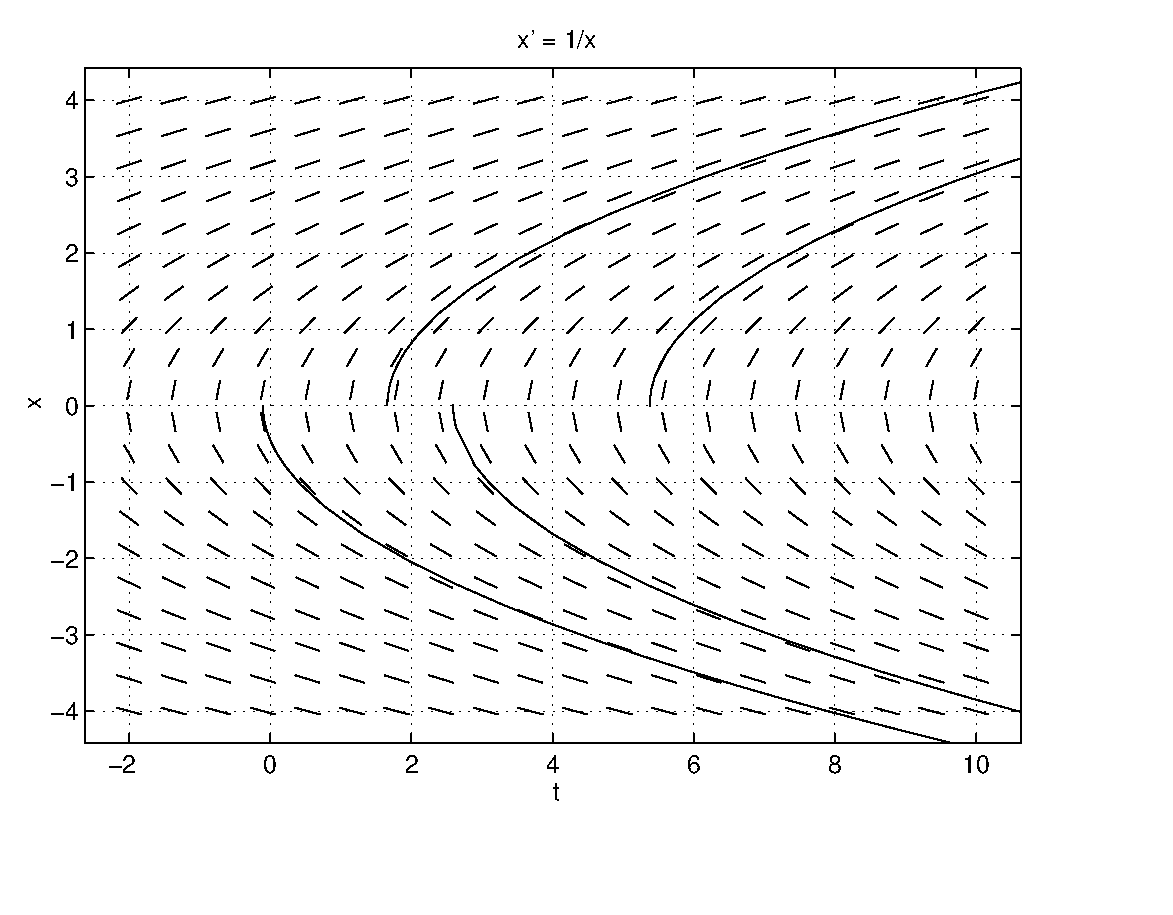
\psfig{file=exfigure/14-1-11aa.eps,width=2.75in}
                       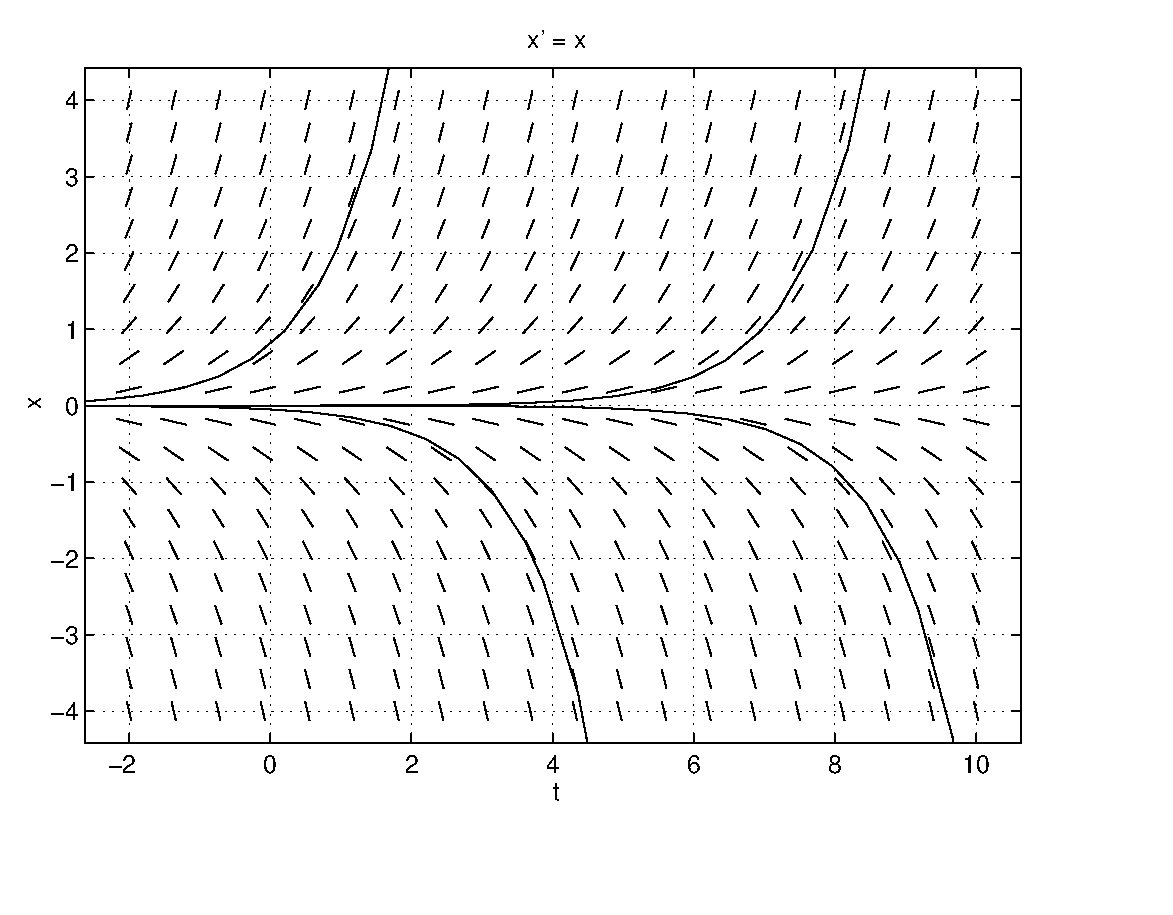
\psfig{file=exfigure/14-1-11ab.eps,width=2.75in}}
                \exercaptwo{c14.1.11a}
\end{figure}

\end{solution}
\end{exercise}
\begin{exercise} \label{c14.1.11b}
$\dps\frac{dx}{dt} = \frac{1}{tx}$.

\begin{solution}
Figure~\ref{c14.1.11b} shows several trajectories of the
differential equation.  Let $x_0 = x(t_0)$ be the initial condition of
a solution.  All solutions with $t_0 > 0$ limit on $x = 0$ in backward time,
and all solutions with $t_0 < 0$ limit on $x_0$ in forward time.  In the
other direction, all solutions with $x_0 > 0$ go to infinity, while all
solutions with $x_0 < 0$ go to negative infinity.

\begin{figure}[htb]
                       \centerline{%
                       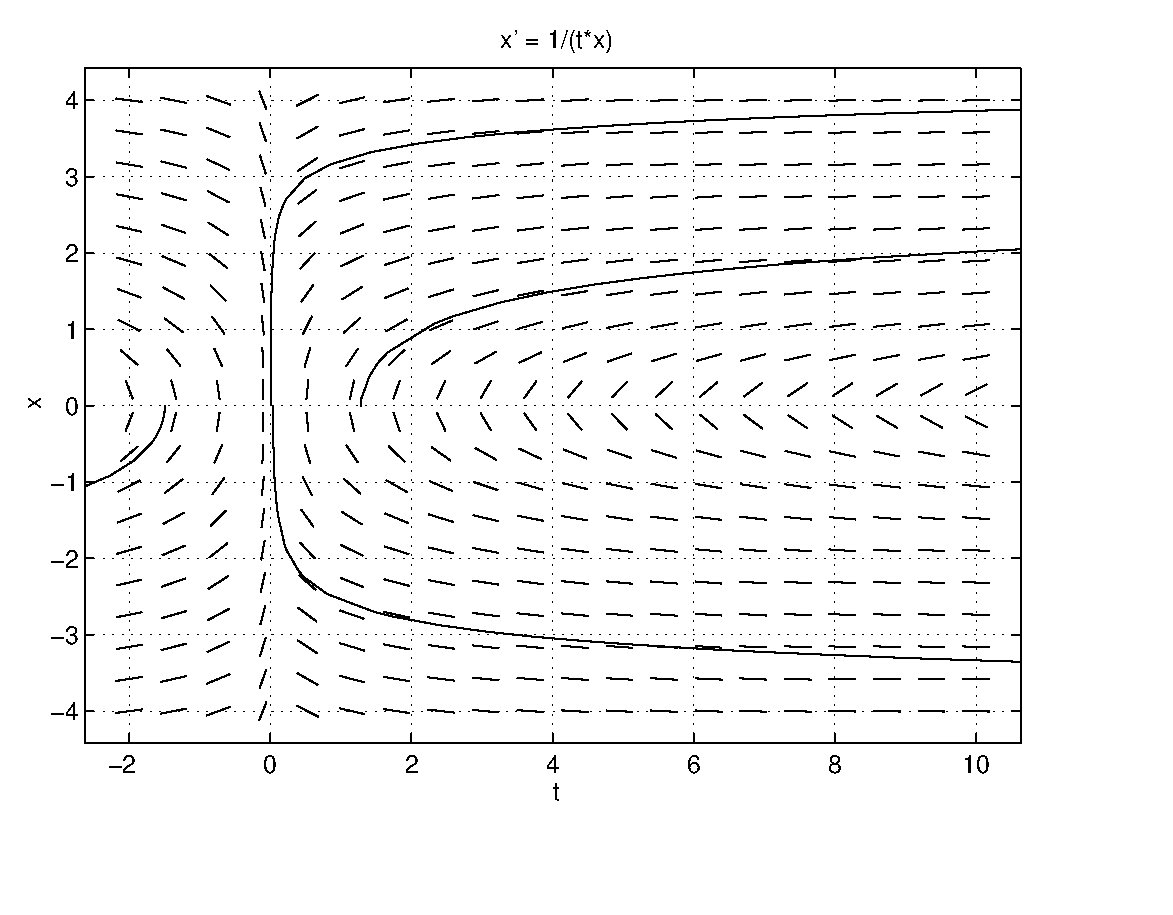
\psfig{file=exfigure/14-1-11b.eps,width=3.0in}}
                \exercap{c14.1.11b}
\end{figure}

\end{solution}
\end{exercise}
\begin{exercise} \label{c14.1.11c}
$\dps\frac{dx}{dt} = \sin(tx)$.

\begin{solution}
Figure~\ref{c14.1.11c} shows several trajectories of the
differential equation.  The equation has a constant solution at $x(t)
= x_0 = 0$.

\begin{figure}[htb]
                       \centerline{%
                       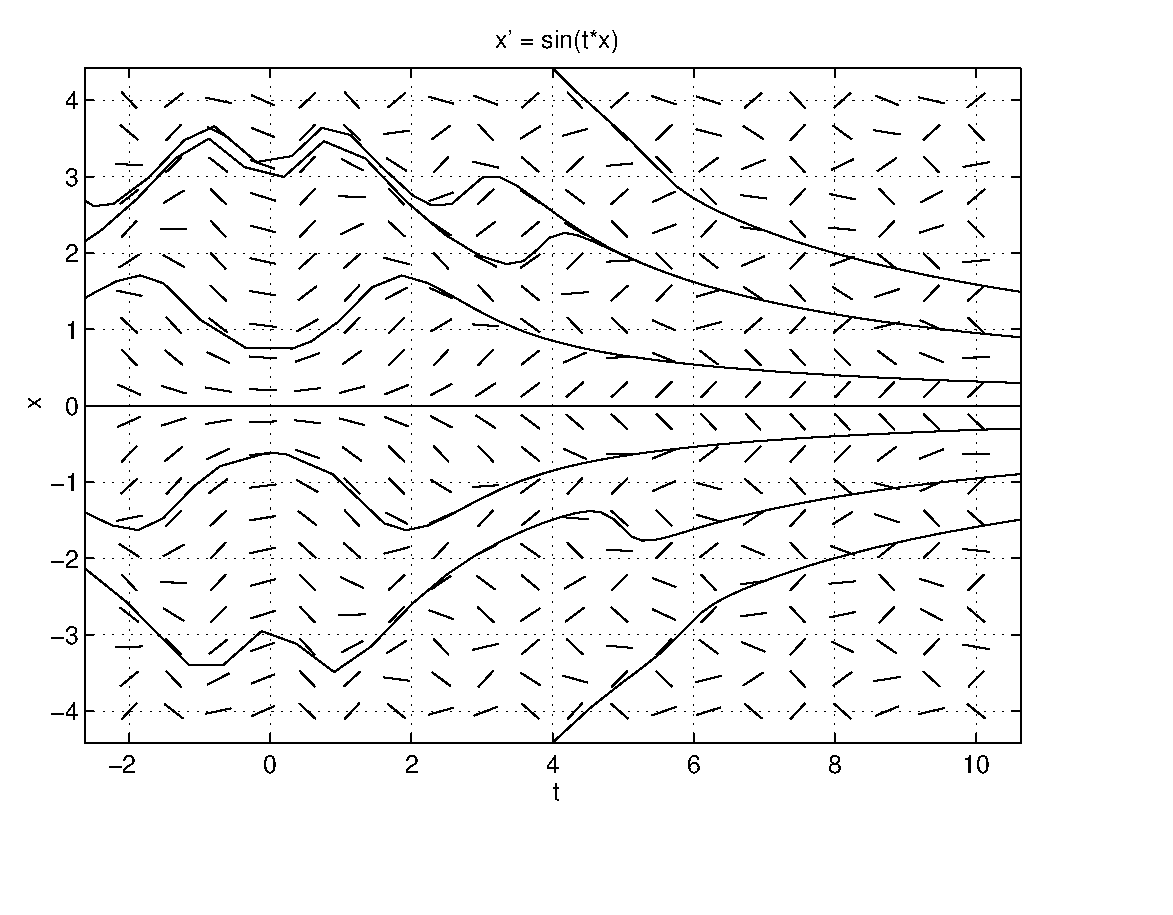
\psfig{file=exfigure/14-1-11c.eps,width=3.0in}}
                \exercap{c14.1.11c}
\end{figure}

\end{solution}
\end{exercise}
\begin{exercise} \label{c14.1.11d}
$\dps\frac{dx}{dt} = t^2 - x^3$.

\begin{solution}
Figure~\ref{c14.1.11d} shows several trajectories of the
differential equation.  All solutions limit on a single trajectory in
forward time.

\begin{figure}[htb]
                       \centerline{%
                       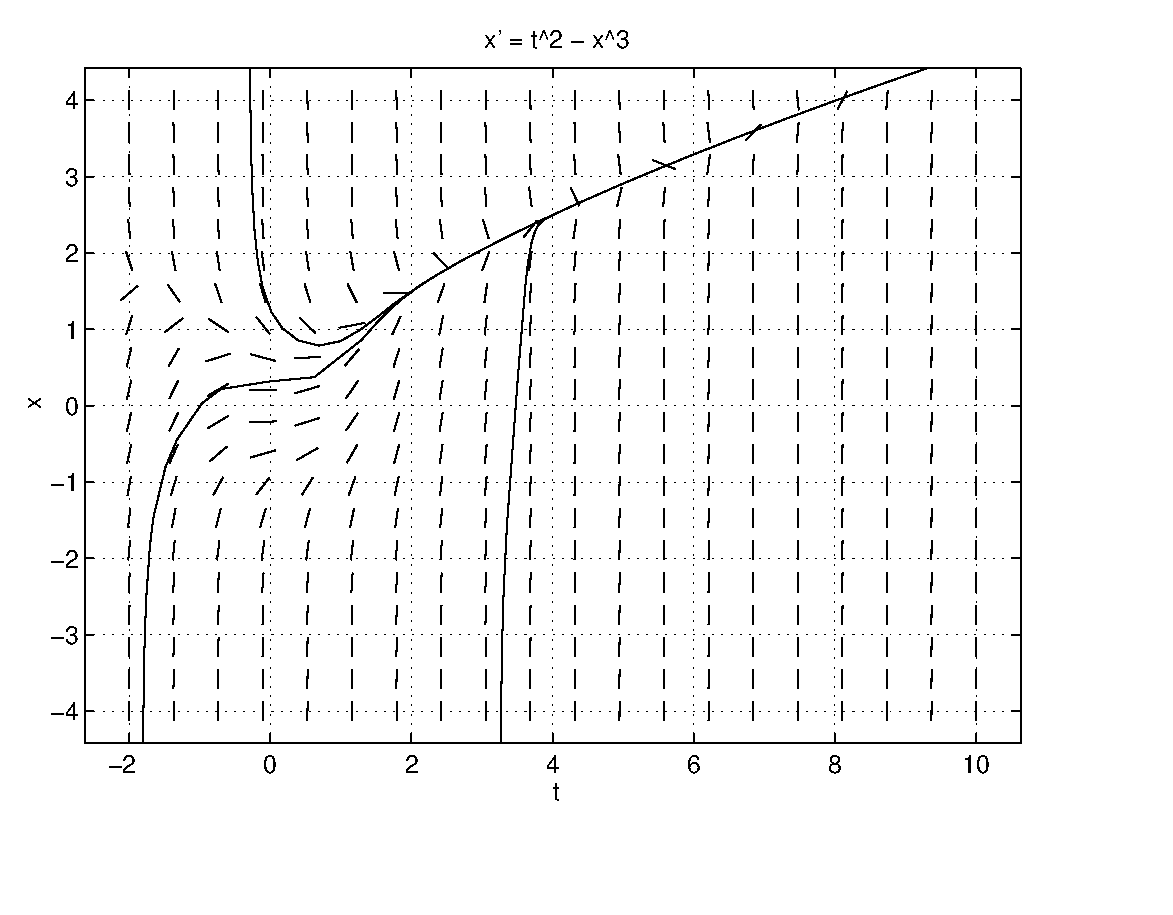
\psfig{file=exfigure/14-1-11d.eps,width=3.0in}}
                \exercap{c14.1.11d}
\end{figure}

\end{solution}
\end{exercise}
\begin{exercise} \label{c14.1.11e}
$\dps\frac{dx}{dt} = x(1-x^2)$.

\begin{solution}
Figure~\ref{c14.1.11e} shows several trajectories of the
differential equation.  The equation has constant solutions $x(t) = 0$,
$x(t) = -1$ and $x(t) = 1$.  All solutions with initial conditions
$x_0 = x(t_0)$ such that $|x_0| < 1$ limit on $x = 0$ in backward time and
limit on $x = 1$ or $x = -1$ in forward time.  All other solutions limit
on $x = 1$ or $x = -1$ in backward time and diverge in forward time.

\begin{figure}[htb]
                       \centerline{%
                       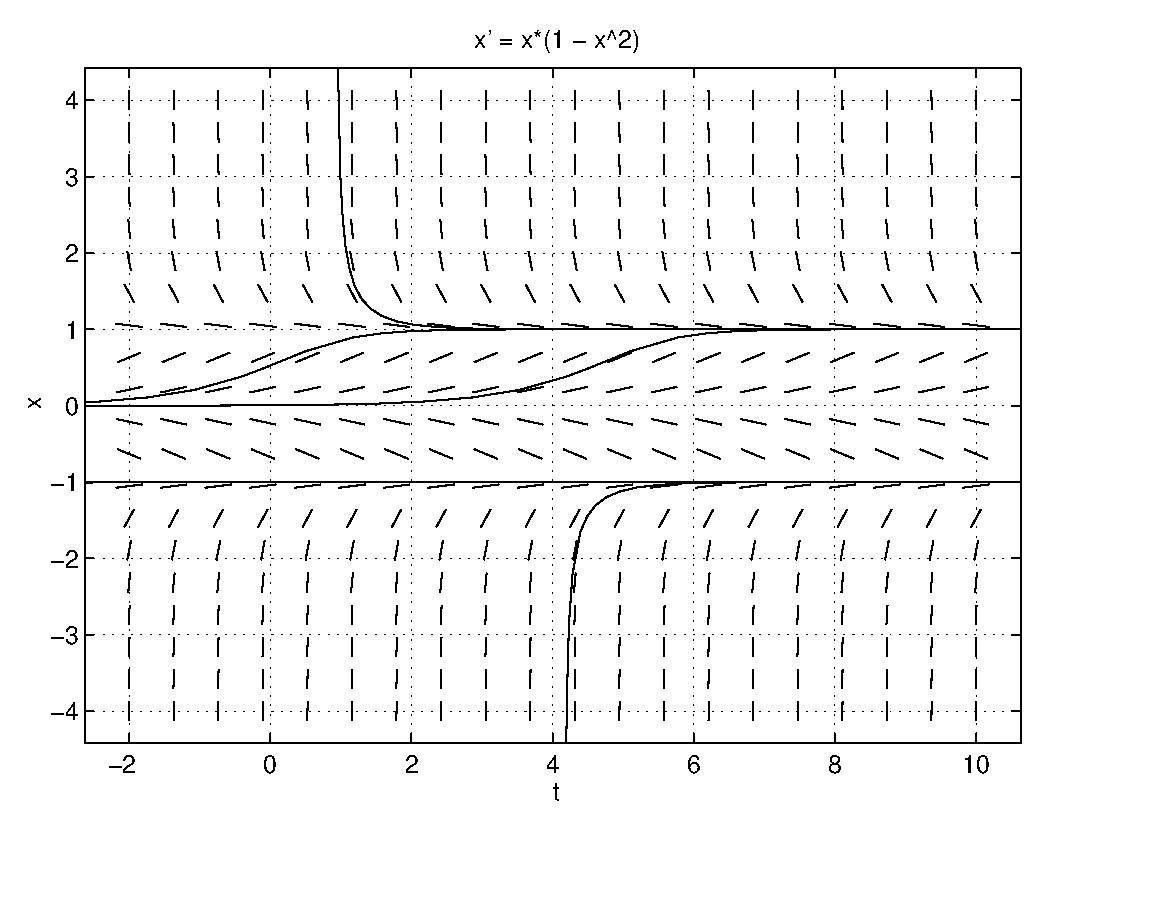
\psfig{file=exfigure/14-1-11e.eps,width=3.0in}}
                \exercap{c14.1.11e}
\end{figure}


\end{solution}
\end{exercise}
\begin{exercise} \label{c14.1.11f}
$\dps\frac{dx}{dt} = \frac{t}{x^2}$.

\begin{solution}
Figure~\ref{c14.1.11f} shows several trajectories of the
differential equation.

\begin{figure}[htb]
                       \centerline{%
                       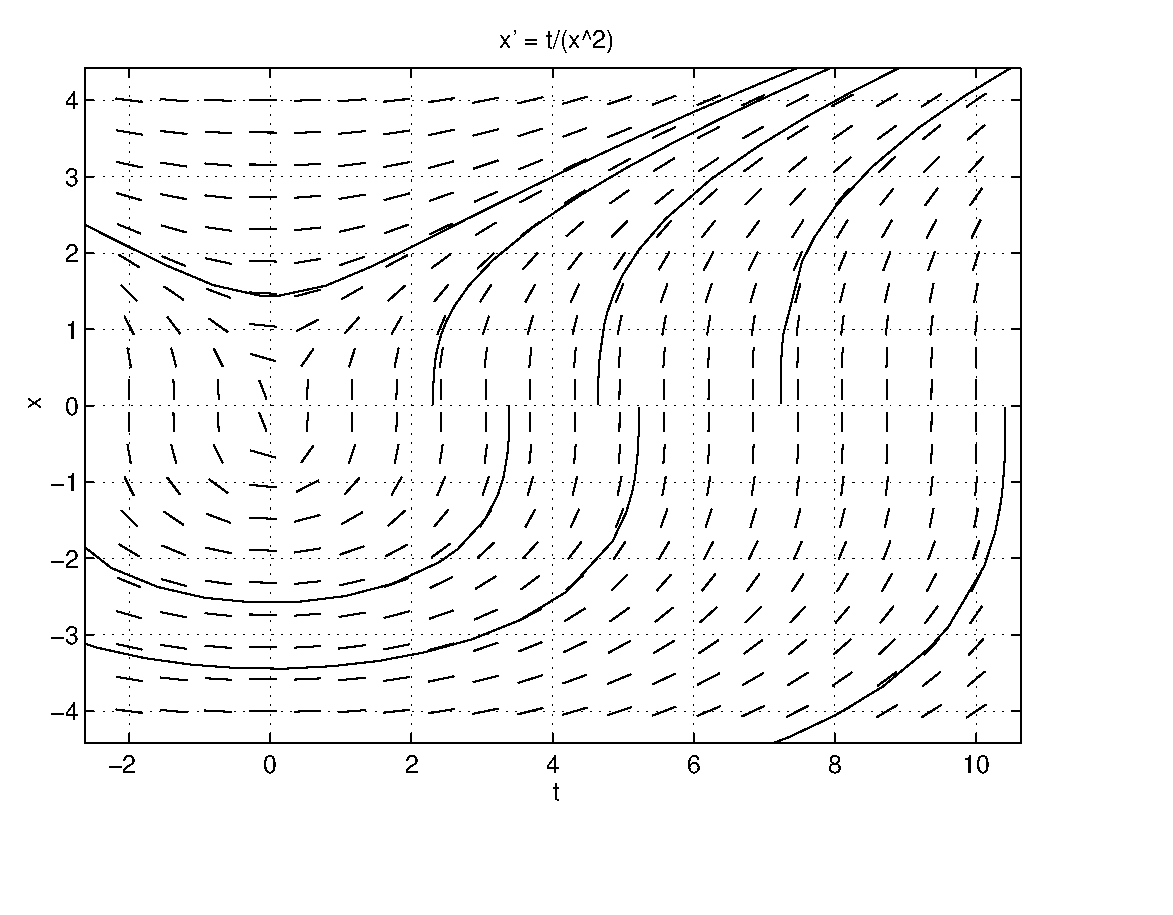
\psfig{file=exfigure/14-1-11f.eps,width=3.0in}}
                \exercap{c14.1.11f}
\end{figure}

\end{solution}
\end{exercise}
\end{document}
